\documentclass[a4paper,12pt]{amsart}
\input epsf
\usepackage{epsfig}
\usepackage{amsmath}
\usepackage{subcaption}

\DeclareMathAlphabet\mathbold{OML}{cmm}{b}{it}
\textheight=8.75in
\textwidth=6in
\oddsidemargin=-0.1in
\evensidemargin=-0.1in
\vsize 8.2in
% Equation numbering
\numberwithin{equation}{section}
 
\newtheorem{theorem}{Theorem}[section]
\newtheorem{lemma}{Lemma}[section]
\newtheorem{remark}{Remark}[section]
\newtheorem{corollary}{Corollary}[section]
\newtheorem{definition}{Definition}[section]
\newtheorem{algorithm}{Algorithm}[section]
\newtheorem{assumption}{Assumption}[section]
\newtheorem{example}{Example}[section]
\newtheorem{proposition}{Proposition}[section]





\newcommand{\curl}{\operatorname{curl}}
\renewcommand{\div}{\operatorname{div}}
\newcommand{\Div}{\operatorname{Div}}
\newcommand{\trace}{\operatorname{tr}}
\newcommand{\diag}{\operatorname{diag}}


\def\b1{{\mathbf 1}}
\def\bv{{\mathbf v}}
\def\bu{{\mathbf u}}
\def\bw{{\mathbf w}}
\def\bb{{\mathbf b}}
\def\bc{{\mathbf c}}
\def\bff{{\mathbf f}}
\def\bg{{\mathbf g}}
\def\bh{{\mathbf h}}
\def\br{{\mathbf r}}
\def\bs{{\mathbf s}}
\def\bd{{\mathbf d}}
\def\be{{\mathbf e}}
\def\bp{{\mathbf p}}
\def\bq{{\mathbf q}}
\def\bx{{\mathbf x}}
\def\by{{\mathbf y}}
\def\bz{{\mathbf z}}
\def\bn{{\mathbf n}}
\def\bbf{{\mathbf f}}
\def\bB{{\mathbf B}}
\def\bM{{\mathbf M}}
\def\bV{{\mathbf V}}
\def\bU{{\mathbf U}}
\def\bY{{\mathbf Y}}
\def\bF{{\mathbf F}}
\def\bA{{\mathbf A}}
\def\bB{{\mathbf B}}
\def\bC{{\mathbf C}}
\def\bD{{\mathbf D}}
\def\bN{{\mathbf N}}
\def\bT{{\mathbf T}}
\def\bP{{\mathbf P}}
\def\bQ{{\mathbf Q}}
\def\bS{{\mathbf S}}
\def\bR{{\mathbf R}}
 
\def\bepsilon{{\boldsymbol \epsilon}}
\def\balpha{{\boldsymbol \alpha}}
\def\bdelta{{\boldsymbol \delta}}
\def\blambda{{\boldsymbol \lambda}}
\def\bmu{{\boldsymbol \mu}}
 
 
 
%-----------------------------------------------------------------
\renewcommand{\O}{{\mathcal O}}
\newcommand{\Q}{{\mathcal Q}}
\newcommand{\R}{{\mathcal R}}
\newcommand{\A}{{\mathcal A}}
\newcommand{\B}{{\mathcal B}}
\newcommand{\C}{{\mathcal C}}
\newcommand{\D}{{\mathcal D}}
\newcommand{\Sc}{{\mathcal S}}
\newcommand{\F}{{\mathcal F}}
\newcommand{\G}{{\mathcal G}}
\newcommand{\I}{{\mathcal I}}
\newcommand{\J}{{\mathcal J}}
\newcommand{\M}{{\mathcal M}}
\newcommand{\N}{{\mathcal N}}
\newcommand{\X}{{\mathcal X}}
\newcommand{\Y}{{\mathcal Y}}
\newcommand{\calY}{{\mathcal Y}}
\newcommand{\calS}{{\mathcal S}}
\renewcommand{\L}{{\mathcal L}}
\renewcommand{\P}{{\mathcal P}}
 
\newcommand{\vertiii}[1]{{\left\vert\kern-0.25ex\left\vert\kern-0.25ex\left\vert #1 
    \right\vert\kern-0.25ex\right\vert\kern-0.25ex\right\vert}}
 
\newcommand{\V}{\text{\bf V}}
\newcommand{\K}{{\mathcal K}}
\newcommand{\T}{{\mathcal T}}
\newcommand{\E}{{\mathcal E}}

\newcommand{\hatcalK}{\widehat{\mathcal K}}
\newcommand{\hatcalS}{\widehat{\mathcal S}}
\newcommand{\hatA}{\widehat{A}}
%% \newcommand{\grad}{\nabla}
%% \renewcommand{\div}{\text{div}}
%% \renewcommand{\curl}{\text{curl}}
%
%
\def\XVec#1{{\mathbf #1}}
\def\XNorm#1{\left\| #1 \right\|}                       % norm
\def\XIProd#1#2{\left\langle #1 ,~ #2 \right\rangle}    % inner product
 
\def\XM{\mu}
 
\def\XQ{Q}                     % interpolant
\def\Xq#1{\XVec{q}_{#1}}       % rows of Q (interpolation to point #1)
\def\Xu{\XVec{u}}              % unknown vector
\def\Xf{\XVec{f}}              % right-hand-side vector
\def\Xe{\XVec{e}}
\def\Xr{\XVec{r}}
\def\Xx{\XVec{x}}
\def\Xv{\XVec{v}}
\def\Xw{\XVec{w}}
\def\Xn{\XVec{n}}              % normal vector
\def\Xes{\Xe_s}
\def\Xec{\Xe_c}
\def\Xus{\Xu_s}
\def\Xuc{\Xu_c}
\def\Xvs{\Xv_s}
\def\Xvc{\Xv_c}
\def\bone{{\boldsymbol 1}}
\def\bphi{{\boldsymbol \varphi}}
\def\bpsi{{\boldsymbol \psi}}
\def\bPsi{{\boldsymbol \Psi}}
\def\btheta{{\boldsymbol \theta}}
\def\bchi{{\boldsymbol \chi}}
\def\boldeta{{\boldsymbol \eta}}
\def\bolddelta{{\boldsymbol \delta}}
\def\bsigma{{\boldsymbol \sigma}}
\def\btau{{\boldsymbol \tau }}
\def\bxi{{\boldsymbol \xi }}
\def\bdelta{{\boldsymbol \delta}}
 
\def\Nedelec{N\'ed\'elec\ }

\def\bPi{{\boldsymbol \Pi}}
\def\bPhi{{\boldsymbol \Phi}}

\newcommand{\ott}[1]{\bar{#1}}
 

\newcommand{\dt}{\partial_t} 
\newcommand{\om}{\Omega} 

\renewcommand{\arraystretch}{1.2}

\DeclareMathOperator*{\argmin}{argmin}
 
 
\title[A minimization solver for AMR in CFOSLS, report] 
{A minimization solver for AMR in constrained first-order system least-squares, report}

\address{Portland State University}

\keywords{CFOSLS, space-time, adaptive mesh refinement, multilevel algorithms, multigrid}

\begin{document}
 
\begin{abstract}
Adaptive mesh refinement is studied for constrained first-order system least-squares (CFOSLS) formulations for three-dimensional space-time problems. While considering the problem at hand as a minimization problem, we use local functional values as a natural measure of the local error. For solving the arising linear systems, an efficient multilevel algorithm is proposed which minimizes the energy functional over a dynamically constructed hierarchy of mesh levels.

Two test problems are considered, the Laplace equation in an L-shaped domain and the transport equation in $H(\div)-L^2$ formulation.

Efficiency of the proposed refinement strategy is compared numerically to the uniform refinement. In addition to the traditional refinement strategy based on local element errors, a modified strategy which noticeably smoothes out the error distribution is implemented by exploiting supplementary face error indicators.

The results obtained show that ... (about refinement results). Furthermore, the proposed multilevel algorithm outperforms the simpler block-diagonal preconditioners in terms of iteration count significantly.
\end{abstract}
\maketitle

\section{Introduction}

Adaptive mesh refinement is studied for constrained first-order system least-squares (CFOSLS) formulations for three-dimensional space-time problems. The central idea of the considered framework is to minimize the least-squares functional under the divergence constraint which makes the method conservative. Following this idea, we use local functional values as a natural measure of the local errors.

Two test problems are considered, one is the Laplace equation in an L-shaped domain and the second is the transport equation in $H(\div)-L^2$ formulation.

Efficiency of the proposed refinement strategy is compared numerically to the uniform refinement. In addition to the traditional refinement strategy based on local element errors, a modified strategy which noticeably smoothes out the error distribution is implemented by exploiting supplementary face error indicators.

For solving the arising linear systems, an efficient multilevel algorithm is proposed which minimizes the energy functional over a hierarchy of mesh levels. The multilevel algorithm outperforms the simpler block-diagonal preconditioners in terms of iteration count significantly.

The results obtained show that ...

\section{Problem statement}

\textbf{Description of the setup in general terms, applicable to both Laplace and transport.}

%\bigskip
%
%Let $\Omega\subset \mathbb{R}^n$ be an open bounded spatial domain with Lipschitz boundary $\partial \Omega$ and let 
%$\Omega_{T} = \Omega\times (0,T)\subset \mathbb{R}^{n+1}$ be the corresponding space-time domain,  where $T>0$ represents the final time.  
%
%Along the lines of \cite{our_paper_cfosls}, below we give a short overview of the unified CFOSLS formulation for a partial differential equation:
%\begin{align} \label{Problem}
%\div \L(u) := \frac{\partial}{\partial_t} \big(\L_t(u) \big)+ \mathrm{div}_\Xx \big( \L_\Xx (u)\big)& = f(\Xx, t), \qquad \text{ for all } (\Xx,t) \in \Omega_T,
%\end{align}
%where we define the space-time differential operator $\L$ to be
%\[
%\L(u) =  \begin{bmatrix} \L_\Xx(u) \\ \L_t(u) \end{bmatrix}.
%\]
%The definiton of $\L_\Xx(u)$ and $\L_t(u)$ which correspond to the Laplace equation and the transport equation can be found  in Table~\ref{tab:PDE_operators}.
%The operators $\div$ and $\div_\Xx$ stand for the $(n+1)$- and $n$-dimensional divergence operators, i.e., for a $C^1$-vector function $\mathbf{g}(\Xx,t)$ in $\mathbb{R}^{n+1}$ with components
%
%$$
%\mathbf{g} =  \begin{bmatrix} \mathbf{g}^\Xx 
%\\ g^t \end{bmatrix}, \quad 
%\mathbf{g}^\Xx \in \mathbb{R}^{n}, \quad g^t \in \mathbb{R} \quad \, \forall (\Xx,t) \in \Omega_T
%$$
%we can write
%$$
%\div \mathbf{g} = \partial_t g^t + \sum_{i = 1}^{n} \partial_{\Xx_i} \mathbf{g}^{\Xx}_i = \partial_t g^t + \div_\Xx \mathbf{g}^{\Xx}.
%$$
%
%% the space of square-integrable functions in $\Omega_T$ denoted by $L^2(\Omega_T)$ , the space of scalar functions $u$ in $L^2(\Omega_T)$ with $\nabla u$ in $L^2(\Omega_T)^{n+1}$, denoted by $H^1(\Omega_T)$ and the space of vector functions $\bsigma$ in $L^2(\Omega_T)^{n+1} $ with $\div \bsigma$ in $L^2(\Omega_T)$, denoted by $H(\div; \Omega_T)$.  
%
%
%In order to have a well-posed problem for equation \eqref{Problem} we impose boundary conditions on $\partial \Omega_T$ specified in Table~\ref{tab:PDE_operators}. Notice that these ``boundary conditions" on  $\partial \Omega_T$ will contain both initial and boundary conditions in the usual sense of time-dependent PDEs. We will consider additional notations for specific parts of the space-time boundary of $\Omega_T$, namely 
%\[
%\Gamma_0 := \Omega\times\{0\},\quad\Gamma_s := \partial\Omega\times(0, T),\quad\Gamma_D := \Gamma_0\cup\Gamma_s,
%\]
%and, for scalar conservation law, we will also introduce 
%\[
%\Gamma_- := \{\Xx\in\partial\Omega \,|\, \bu\cdot\bn < 0 \}\times(0, T)
%\]
%where $\bu(\Xx,t) : \Omega_T \rightarrow \mathbb{R}^n$ is a given advection vector for which we use standard assumptions that guarantee the well-posedness \cite{evans} of problem \eqref{Problem}. Boundary conditions for  \eqref{Problem} can be formally written as
%\[
%tr (u) = 0,
%\]
%where the actual definitions of the trace operator $tr$ for the different PDEs are listed in Table~\ref{tab:PDE_operators}. For simplicity, we restrict ourselves to homogeneous boundary conditions since the treatment of inhomogeneous boundary conditions is straightforward. 
%\begin{table}[h]
%\caption{Definitions of $\L_\Xx(u)$, $\L_t(u)$, and $tr(u)$ for different PDEs.}
%\label{tab:PDE_operators}
%\begin{tabular}{ |c||c|c|c|} \hline
%PDEs & $\quad \L_\Xx(u) \quad$ & $\quad \L_t(u) \quad$ & $\quad tr(u) \quad$  \\ \hline
%Heat equation & $-\nabla_\Xx u$ & $u$ & $u|_{\Gamma_D}$ \\ \hline
%Conservation law & $\bu u$ & $u$ & $u|_{\Gamma_0\,\cup\,\Gamma_-}$   \\ \hline
%Wave equation & $-\nabla_\Xx u$ & $\partial_t u$ & $[u|_{\Gamma_D}, \,\partial_tu|_{\Gamma_0}]$    \\ \hline
%\end{tabular}
%\end{table}
%
%\subsection{Constrained space-time formulation} 
%Following \cite{neumueller_vassilevski_villa} we rewrite equation \eqref{Problem} as a first-order system by introducing a new variable $\bsigma := \L(u)$, 
%obtaining 
%\begin{equation}
%\begin{array}{c}
%\bsigma - \L(u)  = 0,  \\ 
%\div \bsigma = f. 
%\end{array}
%\label{eq:fos} 
%\end{equation}
%
%We will also make use of the following well-known functional spaces: $L^2(\Omega_T)$, the space of square-integrable functions in $\Omega_T$; $H^1(\Omega_T) = \{ u \in L^2(\Omega_T) : \, \nabla u \in L^2(\Omega_T)^{n+1} \} $; $H(\div; \Omega_T) = \{ \bsigma \in L^2(\Omega_T)^{n+1} : \, \div \bsigma \in L^2(\Omega_T) \}$ and omit $\Omega_T$ for the sake of brevity. Also, we denote by  $(\cdot,\cdot)$ the inner product with respect to scalar and vector $L^2$, and by $\|\cdot \|$ the corresponding norm. From now on we will understand all differential operators in the weak sense. %, and $\|\cdot\|_K$ will denote a $K$-weighted $L^2(\Omega_T)$ norm, where $K$ is a symmetric positive definite matrix.
%
%To formulate the least squares problem  we  consider the following spaces with weakly imposed boundary conditions:
%\begin{equation}
%\begin{split}
%R & := \{\,\btheta \in H(\div) \;|\; tr^\sigma(\btheta) = 0\,\};\\
%V & := \{\,v \in H^1 \;|\; tr^u(v) = 0\,\},\\
%\end{split}
%\label{eq:spaces}
%\end{equation}
%where the definitions of the trace operators $tr^{\sigma}$ and $tr^u$ are given in Table~\ref{tab:FOSLS_operators}. These trace operators are well defined, see \cite{gatica}. 
%
%\begin{table}[h]
%\caption{Definitions of $tr^{\sigma}(\bsigma)$, and $tr^u(u)$ for the different PDEs.}
%\label{tab:FOSLS_operators}
%\begin{tabular}{ |c||c|c|} \hline
%PDEs & $\quad tr^{\sigma}(\bsigma) \quad$ & $\quad tr^u(u) \quad$  \\ \hline
%Heat equation & N/A & $u|_{\Gamma_D}$ \\ \hline
%Conservation law  & N/A & $u|_{\Gamma_0\,\cup\,\Gamma_-}$ \\ \hline
%Wave equation     &  $(\bsigma\cdot\bn)|_{\Gamma_0}$ & $u|_{\Gamma_D}$  \\ \hline
%\end{tabular}
%\end{table}
%
%Then, for any given $f\in L^2$ the FOSLS functional for problem \eqref{eq:fos} 
%\begin{align}
%J(\bsigma, u) = \left\| \bsigma - \L(u) \right\|^2 + \| f-\div \bsigma \| ^2 \label{pfunctional}
%\end{align} 
%is well defined in $R \times V$.
%Now, the constrained space-time first-order system least squares (CFOSLS) problem is to find the minimizer of the functional \eqref{pfunctional} 
%under the constraint given by the conservation equation:
%\begin{equation}
%(\bsigma, u) = \argmin_{(\btheta, v)\in R\times V} J(\btheta, v) \;\text{ subject to } \, \div \bsigma = f. 
%\label{eq:minimization}
%\end{equation}
%The constraint is imposed in a weak sense by introducing a Lagrange multiplier from $L_2$. Notice that because the constraint enforces $f-\div \bsigma = 0$, we can omit the second term $\| f-\div \bsigma \| ^2$ in the functional \eqref{pfunctional} in our CFOSLS formulation.
%
%
%\subsection{Variational CFOSLS formulation} 
%For the system \eqref{eq:fos} we define the operator
%\[ 
%\A(\bsigma, u ) = \bsigma -\L(u).
%\]
%It is well known that the minimizer of the constrained minimization problem \eqref{eq:minimization} is characterized by the first order (or Karush-Kuhn-Tucker) optimality condition, which leads in our case to the following saddle point system: 
%
%Find $(\bsigma, u) \in R\times V$ and $\lambda \in L^2$ such that 
%\begin{equation}
%\begin{array}{lll}
%\big(\A(\bsigma, u), \A(\btheta, v) \big) + (\lambda, \mathrm{div}\,  \btheta) & = 0  & \;\forall\; (\btheta, v) \in R\times V,     \\
%( \div  \bsigma,\mu )  &= (f, \mu) &  \;\forall\;  \mu\in L^2.
%\end{array}
%\label{eq:kkt_system}
%\end{equation} 
%%where
%%\begin{align*}
%% H_*(\Omega_T) 
%% &=\{ u \in L^2(0,T: H^1_0(\Omega)): u(x,0) = 0  \text{ for all } x \in \om\} 
%%\end{align*}
%
%The continuity of the bilinear form corresponding to the operator $\A$ is obvious due to the choice of spaces $R$ and $V$. Also, this form can be considered to be weakly-coercive in the sense of the definition given in \cite{AdlerVassilevski}.
%
%\begin{remark}
%A traditional variational FOSLS formulation would be written in our notations as:
%
%Find $(\bsigma, u) \in R\times V$ such that 
%\[
%\big(\A(\bsigma, u ), \A(\btheta, v) \big) + \big( \div \bsigma, \div \btheta \big) = \big(f, \div \btheta\big) \qquad \;\forall\; (\btheta, v) \in R\times V.
%\]
%\end{remark}
%
%\begin{remark}\label{rmk:complicate}
%Notice that, since $u$ belongs to $H^1$, for the scalar conservation law we can consider a different second term $\| \div (\bu u) - f \|^2$ in the FOSLS functional \eqref{pfunctional}. Then we will have an extra weighted diffusion term $(\bu  \, \nabla_x u, \bu \, \nabla_x u)$ for $u$ (which already exists for heat and wave equations due to the definition of $\bsigma$ for these problems).
%
%Then, instead of \eqref{eq:kkt_system}, we will have the following
% system:
%\begin{equation}
%\begin{array}{lll}
%\big(\A_+(\bsigma, u), \A_+(\btheta, v) \big) + (\lambda, \mathrm{div}\,  \btheta) & = \big( f, \div (\bu v) \big)  & \;\forall\; (\btheta, v) \in R\times V,     \\
%( \div  \bsigma,\mu )  &= (f, \mu) &  \;\forall\;  \mu\in L^2.
%\end{array}
%\label{eq:kkt_system_compl}
%\end{equation} 
%with
%\begin{equation}
%\A_+(\bsigma, u) = \begin{bmatrix} \A(\bsigma, u) \\ \div (\bu u) \end{bmatrix}.
%\label{eq:Adefine}
%\end{equation}
%We use this modified formulation when we consider scalar conservation law with $u\in~H^1$.
%\end{remark}
%
%As one can notice, in equation \eqref{eq:kkt_system}  we seek for $u$ in $V \subset H^1$. However, in case of the scalar conservation law we can also allow $u$ to  have less regularity. This is due to the fact that unlike the other example problems,  the definition of $\mathcal{L}(u)$ does not involve any derivatives of $u$.  
%%
%%First we consider space \textcolor{blue}{ (why $\tilde V $, if it is not defined later maybe we can erase it)}  $\tilde{V} = L^2(\Omega_T)$ instead of $V$ for $u$ and impose the boundary conditions on $\bsigma$: $(\bsigma\cdot\bn)|_{\Gamma_0\,\cup\,\Gamma_-}$ instead of those for $u$ in $H^1$ case.
%Hence, we can obtain a new formulation by seeking $u  \in L^2(\om)$ instead of $V$ and imposing the boundary conditions on $\bsigma$ instead of $u$, i.e. replacing $u|_{\Gamma_0\,\cup\,\Gamma_-}$ with $(\bsigma\cdot\bn)|_{\Gamma_0\,\cup\,\Gamma_-}$. 
%
%Next, as it follows from the first equation of \eqref{eq:fos},  the scalar unknown $u$ can be expressed in terms of $\bsigma$:
%\begin{equation}
%u = \frac1{\bb^T \bb }\bb^T \bsigma,
%\label{eq:S}
%\end{equation}
%where we introduced the space-time vector function
%\[
%\bb = \bb(\Xx,t) := \begin{bmatrix} \bu(\Xx,t) \\ 1 \end{bmatrix}.
%\]
%Notice that $\bb^T\bb \equiv \bu^T\bu+1 \ge 1$, thus $\bb^T\bb$ is a strictly positive function.
%
%Now we substitute \eqref{eq:S} for $u$ in \eqref{eq:kkt_system} and redefine $\A(\bsigma,u)$ in \eqref{eq:kkt_system} to depend on $\bsigma$ only. The final variational problem then reads as:
%
%Find $\bsigma \in R$ and $\lambda \in L^2$ such that 
%\begin{equation}
%\begin{array}{lll}
%\big( K \bsigma, \btheta \big) + (\lambda, \mathrm{div}\,  \btheta) & = 0  & \;\forall\; \btheta \in R,     \\
%( \div  \bsigma,\mu )  &= (f, \mu) &  \;\forall\;  \mu\in L^2.
%\end{array}
%\label{eq:altkkt_system}
%\end{equation}
%where we have introduced a symmetric positive semi-definite matrix coefficient $K(x,t)$ defined as 
%\begin{equation}
%K :=  I - \frac{1}{\bb^T\bb} \bb \bb^T.
%\end{equation}
%Notice that \eqref{eq:altkkt_system} can be obtained as a variational formulation of the minimization problem for the following modified functional:
%$$
%\tilde{J}(\bsigma) = \left\| \bsigma \right\|_K^2 + \| f- \div \bsigma \| ^2, \label{modfunctional}
%$$
%where $\|\bsigma\|_K$ represents the $K$-weighted $L^2$ seminorm for $\bsigma$. 
%
%\begin{remark}
%One should be careful when considering the alternative formulation \eqref{eq:altkkt_system}. Although it looks similar to a standard mixed formulation for a Laplace equation, the presense of the matrix weight $K$ makes it very different. $K(x,t)$ is rank-deficient (since $K \cdot \bb \equiv 0$) at any point $(\Xx,t)$ but the corresponding global operator is non-singular at the kernel of the divergence operator due to the underlying assumption that the original differential problem is well-posed, which implies, in particular, that the global matrix corresponding to $(K\cdot,\cdot)$ should  be positive definite in the subspace $\{\bsigma \in R : \div \, \bsigma = 0\}$. Local rank deficiency certainly affects the conditioning number of the resulting linear system and makes the problem of finding optimal iterative solvers much more complicated.
%\end{remark}
%
%\begin{remark}
%Once $\bsigma$ is found as a solution to \eqref{eq:altkkt_system}, $u$ can be recovered from the weak form of \eqref{eq:S} if needed.
%\end{remark}


\section{Refinement strategy}
Description of the element error indicators, and a modification with the face error indicators.

Definition of threshold in MFEM:
$$
\mbox{threshold} = \max \left\lbrace \mbox{total error} \cdot \mbox{total error fraction} \cdot n_{el}^{-\frac{1}{p}}, \, \mbox{local error goal} \right\rbrace.
$$

Total error is defined by
$$
\mbox{total error}  = 
\left\{ 
\begin{array}{lc}
\left( \sum_i \left(\mbox{local error i}\right)^p \right)^{1/p}, & p < \infty \\
\max_i \mbox{local error i}, & p = \infty \\
\end{array}
\right.
$$

Default parameter values are:
\begin{itemize}
	\item $\mbox{total error fraction} = 0.5$;
	\item $p = \infty$;
	\item $\mbox{local error goal} = 0.0$.
\end{itemize}

\section{Linear solvers}

\subsection{Block-diagonal preconditioners}

\subsection{Multilevel minimization solver}

\section{Results}

\subsection{Refinement stats?}

\subsection{Comparison to the uniform refinement}

\subsubsection{Laplace}

\begin{table}[h!]
\caption{Uniform refinement, L-shaped domain in $\mathbb{R}^3$, $H(\div)-H^1$ formulation for the Laplace equation}
\label{tab:ur_conv_lshape3D_HdivH1lapl}
\scalebox{.85}{
\begin{tabular}{|c||c|c|c|c|c|} \hline
\#dofs & \#iter 1 & \#iter 2 & $\varepsilon_{\bsigma}$ & $\varepsilon_u$ & FOSLS func value \\ \hline
8231   & 1  & 151 & 0.113 & 0.021  & 5.11e-3 (5.35e-3) \\ \hline
63677  & 10 & 186 & 0.073 & 0.008  & 1.19e-3 (1.25e-3) \\ \hline 
501049 & 11 & 214 & 0.047 & 0.0032 & 2.70e-4 (2.85e-4) \\ \hline 
\end{tabular}}
% minsolver tolerance 1.0e-6
\end{table}
In table \ref{tab:ur_conv_lshape3D_HdivH1lapl} convergence in case of uniform refinement is given for the Laplace equation. Each row of the table corresponds to a refinement level. The second and third columns give the number of iterations of the proposed multilevel solver (using all levels which are available at the current iteration) and the block-diagonal preconditioner for the saddle-point system. The third and fourth column show the relative errors in $L^2$ for $\bsigma$ and $u$.
The last column gives the FOSLS functional value for the computed solution and for the projection of the exact analytical solution (in parentheses).

\begin{table}[h!]
\caption{AMR, L-shaped domain in $\mathbb{R}^3$, $H(\div)-H^1$ formulation for the Laplace equation}
\label{tab:amr_conv_lshape3D_HdivH1lapl}
\scalebox{.85}{
\begin{tabular}{|c||c|c|c|c|c|} \hline
\#dofs & \#iter 1 & \#iter 2 & $\varepsilon_{\bsigma}$ & $\varepsilon_u$ & FOSLS func value \\ \hline
8231   & 1  & 151 & 0.113 & 0.021   & 5.11e-3 (5.35e-3) \\ \hline
8940   & 5  & 152 & 0.104 & 0.016   & 4.37e-3 (4.61e-3) \\ \hline 
10109  & 7  & 157 & 0.094 & 0.014   & 3.81e-3 (4.04e-3) \\ \hline 
10960  & 5  & 157 & 0.088 & 0.012   & 3.48e-3 (3.72e-3) \\ \hline 
12421  & 5  & 155 & 0.082 & 0.011   & 3.03e-3 (3.27e-3) \\ \hline 
16678  & 8  & 161 & 0.074 & 0.008   & 2.32e-3 (2.51e-3) \\ \hline 
17849  & 4  & 163 & 0.072 & 0.0078  & 2.19e-3 (2.38e-3) \\ \hline 
18275  & 3  & 164 & 0.071 & 0.0077  & 2.15e-3 (2.34e-3) \\ \hline 
23488  & 6  & 166 & 0.067 & 0.0071  & 1.77e-3 (1.94e-3) \\ \hline 
24068  & 4  & 167 & 0.066 & 0.070   & 1.74e-3 (1.91e-3) \\ \hline 

29566  & 7  & 170 & 0.063 & 0.0063  & 1.48e-3 (1.63e-3) \\ \hline 
32807  & 4  & 174 & 0.061 & 0.006   & 1.37e-3 (1.51e-3) \\ \hline 
34472  & 4  & 177 & 0.060 & 0.0056  & 1.31e-3 (1.44e-3) \\ \hline 
41002  & 5  & 186 & 0.058 & 0.0052  & 1.15e-3 (1.27e-3) \\ \hline 
50849  & 5  & 187 & 0.055 & 0.0049  & 9.9e-4  (1.1e-3) \\ \hline 
53068  & 3  & 187 & 0.054 & 0.0047  & 9.56e-4 (1.06e-3) \\ \hline 
58231  & 5  & 187 & 0.053 & 0.0046  & 8.93e-4 (9.94e-4) \\ \hline 
69791  & 5  & 188 & 0.052 & 0.0045  & 7.94e-4 (8.87e-4) \\ \hline 
72699  & 4  & 187 & 0.051 & 0.0044  & 7.67e-4 (8.59e-4) \\ \hline 
76852  & 4  & 190 & 0.050  & 0.0043 & 7.37e-4 (8.28e-4) \\ \hline 
\end{tabular}}
% minsolver tolerance 1.0e-6
% conservative strategy, 0.95
% beta = infty
\end{table}
In table \ref{tab:amr_conv_lshape3D_HdivH1lapl} (cf. with \ref{tab:ur_conv_lshape3D_HdivH1lapl}) convergence in case of adaptive mesh refinement refinement is given for the Laplace equation.

\subsubsection{Transport}

\begin{table}[h!]
\caption{Uniform refinement, rotating Gaussian hill, $H(\div)-L^2$ formulation for the transport equation}
\label{tab:ur_conv_3D_HdivL2tran}
\scalebox{.85}{
\begin{tabular}{|c||c|c|c|c|c|} \hline
\#dofs & \#iter 1 & \#iter 2 & $\varepsilon_{\bsigma}$ & FOSLS func value \\ \hline
1248   & 1    & 174  & 0.96 & 2.48e-5 (2.8e-3) \\ \hline
9600   & 154  & 361  & 0.99 & 3.15e-5 (8.05e-4) \\ \hline
75264  & 293  & 535  & 0.75 & 5.2e-5  (2.02e-4) \\ \hline 
595968 & 500+ & 1174 & 0.57 & 1.35e-5 (3.71e-5) \\ \hline 
\end{tabular}}
% minsolver tolerance 1.0e-8
\end{table}
In table \ref{tab:ur_conv_3D_HdivL2tran} convergence in case of uniform refinement is given for the transport equation.
The last column gives the FOSLS functional value for the computed solution and for the projection of the exact analytical solution (in parentheses). As one can notice, the results are significantly worse than in case of the Laplace equation. There are at least two reasons for that. First, the exact solution, as it is typical for hyperbolic problems, is essentially discontinuous, with very steep gradients and thus is less regular than the solution of the Laplace test.
Second, one should not forget the hyperbolic nature of the problem at hand. It makes the functional converge much slower and thus worsens the behavior of the linear solvers, due to the presence of the semi-definite matrix weight in the mass matrix in \ref{eq:something}. 

\begin{table}[h!]
\caption{AMR, rotating Gaussian hill $\mathbb{R}^3$, $H(\div)-L^2$ formulation for the transport equation}
\label{tab:amr_conv_3D_HdivL2tran}
\scalebox{.85}{
\begin{tabular}{|c||c|c|c|c|} \hline
\#dofs & \#iter 1 & \#iter 2 & $\varepsilon_{\bsigma}$ & FOSLS func value \\ \hline
9600  & 1  & 361 & 0.96  & 3.15e-5 (8.05e-4) \\ \hline
10563 & 23 & 351 & 0.85  & 1.67e-4 (8.1e-4) \\ \hline
11391 & 23 & 384 & 0.81  & 1.59e-4 (7.1e-4) \\ \hline
12075 & 21 & 391 & 0.81  & 1.51e-4 (6.89e-4) \\ \hline
13303 & 22 & 399 & 0.78  & 1.44e-4 (5.63e-4) \\ \hline
13981 & 22 & 427 & 0.78  & 1.35e-4 (5.47e-4) \\ \hline
15895 & 36 & 431 & 0.76  & 1.21e-4 (5.08e-4) \\ \hline
17335 & 29 & 389 & 0.75  & 1.13e-4 (4.77e-4) \\ \hline
18867 & 22 & 389 & 0.75  & 1.04e-4 (4.58e-4) \\ \hline

23042 & 79 & 484 & 0.70  & 8.85e-5 (3.52e-4) \\ \hline
24116 & 50 & 498 & 0.69  & 8.52e-5 (3.33e-4) \\ \hline
30167 & 50 & 525 & 0.67  & 7.11e-5 (2.83e-4) \\ \hline
32907 & 91 & 569 & 0.65  & 6.61e-5 (2.47e-4) \\ \hline
33816 & 71 & 591 & 0.64  & 6.47e-5 (2.42e-4) \\ \hline

38570 & 69 & 625 & 0.62  & 5.89e-5 (2.0e-4) \\ \hline
42241 & 68 & 526 & 0.60  & 5.48e-5 (1.81e-4) \\ \hline
47698 & 68 & 669 & 0.59  & 5.03e-5 (1.65e-4) \\ \hline
50338 & 65 & 586 & 0.58  & 4.84e-5 (1.59e-4) \\ \hline

60598 & 78 & 741 & 0.56  & 4.25e-5 (1.38e-4) \\ \hline
61940 & 76 & 717 & 0.56  & 4.19e-5 (1.38e-4) \\ \hline

\end{tabular}}
% minsolver tolerance 1.0e-8
% conservative strategy, 0.95
% beta = infty
\end{table}
In table \ref{tab:amr_conv_3D_HdivL2tran} (cf. with \ref{tab:ur_conv_3D_HdivL2tra}) convergence in case of adaptive mesh refinement refinement is given for the transport equation.

\begin{table}[h!]
\caption{AMR, rotating Gaussian hill $\mathbb{R}^3$, $H(\div)-L^2$ formulation for the transport equation, coarser starting mesh}
\label{tab:amr2_conv_3D_HdivL2tran}
\scalebox{.85}{
\begin{tabular}{|c||c|c|c|c|} \hline
\#dofs & \#iter 1 & \#iter 2 & $\varepsilon_{\bsigma}$ & FOSLS func value \\ \hline
1248  & 1  & 174 & 0.99  & 2.48e-5 (2.8e-3) \\ \hline
1469  & 10 & 189 & 0.99  & 7.76e-5 (3.28e-3) \\ \hline
2221  & 10 & 214 & 0.92  & 3.77e-4 (2.73e-3) \\ \hline
3195  & 19 & 239 & 0.86  & 4.16e-4 (1.54e-3) \\ \hline
3915  & 18 & 253 & 0.85  & 3.43e-4 (1.43e-3) \\ \hline
5545  & 39 & 290 & 0.83  & 2.49e-4 (9.16e-4) \\ \hline
6408  & 26 & 302 & 0.82  & 2.34e-4 (8.45e-3) \\ \hline
7601  & 28 & 330 & 0.81  & 2.05e-4 (7.28e-4) \\ \hline
7908  & 26 & 334 & 0.80  & 1.96e-4 (7.99e-4) \\ \hline

11584 & 47 & 386 & 0.77  & 1.48e-4 (6.24e-4) \\ \hline
16646 & 84 & 505 & 0.74  & 1.13e-4 (5.34e-4) \\ \hline
17078 & 66 & 490 & 0.72  & 1.11e-4 (5.2e-4) \\ \hline
19317 & 56 & 511 & 0.71  & 1.00e-4 (4.31e-4) \\ \hline
24727 & 59 & 570 & 0.69  & 8.34e-5 (3.41e-4) \\ \hline

28957 & 87 & 623 & 0.65  & 7.42e-5 (2.88e-4) \\ \hline
33100 & 81 & 641 & 0.64  & 6.78e-5 (2.48e-4) \\ \hline
35521 & 80 & 660 & 0.62  & 6.47e-5 (2.31e-4) \\ \hline
41028 & 77 & 684 & 0.61  & 5.84e-5 (2.06e-4) \\ \hline

48368 & 81 & 747 & 0.6   & 5.26e-5 (1.84e-4) \\ \hline
55482 & 81 & 779 & 0.59  & 4.77e-5 (1.69e-4) \\ \hline

\end{tabular}}
% minsolver tolerance 1.0e-8
% conservative strategy, 0.95
% beta = infty
\end{table}

\textbf{Pictures}

\subsection{Solver comparison} ~\\

\textbf{Block-diagonal preconditioner}

\textbf{Multilevel solver}


%For example, for the first two tables, total error fraction for the adaptive mesh refinement was 0.95.
%This means, that with default values for the rest of parameters,
%a refinement criteria was
%$$
%\mbox{local error i} \geq 0.95 \max_j \mbox{local error j}
%$$
%
%For the L-shaped domain, this strategy leads to the following refinement statistics:
%
%\begin{table}[h!]
%\caption{AMR stats, L-shaped domain in $\mathbb{R}^3$, $H(\div)-H^1$ formulation for the Laplace equation}
%\label{tab:amr_stats_lshape3D_HdivH1lapl}
%\scalebox{.85}{
%\begin{tabular}{|c||c|c|c|c|} \hline
%\#dofs & $n_{\mbox{el, marked}}$ & $\mbox{marked el,} \%$ & $n_{\mbox{el, new}}$ & $\mbox{new el,} \%$ \\ \hline
%63677  & 6    & 0.03  & 362  & 1.86 \\ \hline 
%64861  & 1    & 0.005 & 85   & 0.43 \\ \hline
%65139  & 6    & 0.03  & 694  & 3.49 \\ \hline
%67381  & 2    & 0.01  & 88   & 0.43 \\ \hline
%67678  & 2    & 0.01  & 114  & 0.55 \\ \hline
%68053  & 2    & 0.01  & 174  & 0.84 \\ \hline
%68626  & -    & -     & -    & -    \\ \hline
%\end{tabular}}
%%checked
%\end{table}
%
%\begin{table}[h!]
%\caption{AMR stats, L-shaped domain in $\mathbb{R}^3$, $H(\div)-H^1$ formulation for the Laplace equation}
%\label{tab:amr_stats_lshape3D_HdivH1lapl}
%\scalebox{.85}{
%\begin{tabular}{|c||c|c|c|c|c|c|} \hline
%\#dofs & \#iter1 & \#iter2 & $\varepsilon_{\bsigma}$ & $\varepsilon_u$ & funct & funct for $\pi exsol$ \\ \hline
%63677  & 1           & 1 & 0.073 & 0.008  & 0.00029 & 0.00034 \\ \hline 
%64861  & 1+5         & 2 & 0.068 & 0.0069 & 0.00025 & 0.00028 \\ \hline 
%65139  & 1+5+4       & 2 & 0.067 & 0.0068 & 0.00024 & 0.00027 \\ \hline
%67381  & 1+5+4+7     & 3 & 0.062 & 0.0056 & 0.0002  & 0.00023 \\ \hline
%67678  & 1+5+4+7+3   & 2 & 0.061 & 0.0054 & 0.00019 & 0.00022 \\ \hline
%68053  & 1+5+4+7+3+5 & 2 & 0.060 & 0.0053 & 0.00019 & 0.00022 \\ \hline
%
%\end{tabular}}
%\end{table}
%
%Notations: \#iter1 is for the setup with re-solving from coarsest to finest level each time, \#iter2 is for simple minimization solver at the finest level. The numbers are the numbers of V-cycles so that the first number (1) in column 2 (\#iter1) corresponds to the single iteration (solution of the global system for a correction) at the coarsest level.
%
%Next, the same test but with total error fraction equal to 0.8.
%
%\begin{table}[h!]
%\caption{AMR stats, L-shaped domain in $\mathbb{R}^3$, $H(\div)-H^1$ formulation for the Laplace equation}
%\label{tab:amr_stats_lshape3D_HdivH1lapl}
%\scalebox{.85}{
%\begin{tabular}{|c||c|c|c|c|} \hline
%\#dofs & $n_{\mbox{el, marked}}$ & $\mbox{marked el,} \%$ & $n_{\mbox{el, new}}$ & $\mbox{new el,} \%$ \\ \hline
%63677  & 9    & 0.05  & 623  & 3.2 \\ \hline 
%65709  & 15   & 0.07  & 859  & 4.2 \\ \hline
%68501  & 50   & 0.24  & 3290 & 15.7 \\ \hline
%79092  & 42   & 0.17  & 2272 & 9.4 \\ \hline
%86468  & 10   & 0.04  & 949  & 3.6  \\ \hline
%89541  & 111  & 0.4   & 6584 & 23.9 \\ \hline
%110743 & -    & -     & -    & -    \\ \hline
%\end{tabular}}
%%checked
%\end{table}
%
%\begin{table}[h!]
%\caption{AMR stats, L-shaped domain in $\mathbb{R}^3$, $H(\div)-H^1$ formulation for the Laplace equation}
%\label{tab:amr_stats_lshape3D_HdivH1lapl}
%\scalebox{.85}{
%\begin{tabular}{|c||c|c|c|c|c|} \hline
%\#dofs & \#iter & $\varepsilon_{\bsigma}$ & $\varepsilon_u$ & funct & funct for $\pi exsol$ \\ \hline
%63677  & 1           & 0.073 & 0.008  & 0.00029 & 0.00034 \\ \hline 
%65709  & 1+6         & 0.066 & 0.0065 & 0.00023 & 0.00026 \\ \hline 
%68501  & 1+6+7       & 0.059 & 0.0052 & 0.00019 & 0.00022 \\ \hline
%79092  & 1+6+7+5     & 0.052 & 0.0036 & 0.00013 & 0.00015 \\ \hline
%86468  & 1+6+7+5+8   & 0.048 & 0.0031 & 0.00010 & 0.00013 \\ \hline
%89541  & 1+6+7+5+8+4 & 0.047 & 0.0031 & 0.00009 & 0.00012 \\ \hline
%\end{tabular}}
%\end{table}
%
%\begin{table}[h!]
%\caption{Uniform refinement, L-shaped domain in $\mathbb{R}^3$, $H(\div)-H^1$ formulation for the Laplace equation}
%\label{tab:ur_stats_lshape3D_HdivH1lapl}
%\scalebox{.85}{
%\begin{tabular}{|c||c|c|c|} \hline
%\#dofs & \#iter & $\varepsilon_{\bsigma}$ & $\varepsilon_u$  \\ \hline
%63677  & 9  & 0.073 & 0.008  \\ \hline 
%501049 & 11 & 0.047 & 0.0032 \\ \hline 
%\end{tabular}}
%\end{table}
%Here a MG preconditioner was used, \#levels = 2 and 3.

\section{Figures}
\begin{figure}[h!]
\centering
\begin{subfigure}[t]{0.49\textwidth}
	\raisebox{-\height}{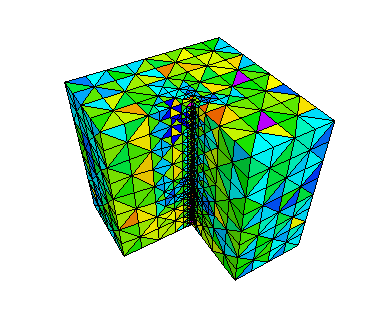
\includegraphics[width=\textwidth]{plots/beta_infinity.png}}
	\caption{$\beta = \infty$}
\end{subfigure}
	\hfill
\begin{subfigure}[t]{0.49\textwidth}
	\raisebox{-\height}{\includegraphics[width=\textwidth]{plots/{beta_1.0}.png}}
	\caption{$\beta = 1.0$}
\end{subfigure}

\begin{subfigure}[t]{0.49\textwidth}
	\raisebox{-\height}{\includegraphics[width=\textwidth]{plots/{beta_0.01}.png}}
	\caption{$\beta = 0.01$}
\end{subfigure}
	\hfill
\begin{subfigure}[t]{0.49\textwidth}
	\raisebox{-\height}{\includegraphics[width=\textwidth]{plots/{beta_0.01}.png}}
	\caption{$\beta = 0.01$}
\end{subfigure}

\begin{subfigure}[t]{0.49\textwidth}
	\raisebox{-\height}{\includegraphics[width=\textwidth]{plots/{beta_0.001}.png}}
	\caption{$\beta = 0.001$}
\end{subfigure}
	\hfill
\begin{subfigure}[t]{0.49\textwidth}
	\raisebox{-\height}{\includegraphics[width=\textwidth]{plots/{beta_0.0001}.png}}
    \caption{$\beta = 0.0001$}
\end{subfigure}

%\subfigure[$\beta = \infty$]{0.49\textwidth}{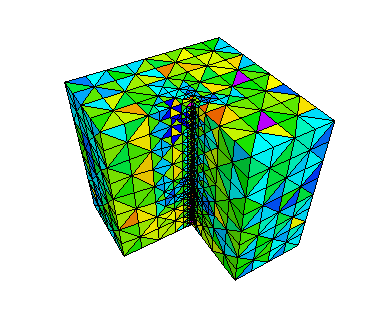
\includegraphics[scale=.6]{plots/beta_infinity.png}}
%\hfill
%%\subfigure[Solver time (log-log plot)]{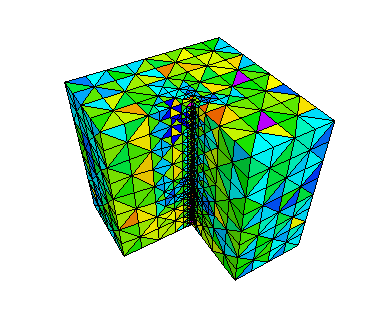
\includegraphics[scale=.08,clip,trim=3.5cm 0 7cm 2cm]{plots/beta_infinity.png}}
%\subfigure[$\beta = 1.0$]{\includegraphics[scale=.6]{plots/{beta_1.0}.png}}

%%\subfigure[$\beta = 0.1$]{\includegraphics[scale=.6]{plots/{beta_0.1}.png}}
%\subfigure[$\beta = 0.01$]{\includegraphics[scale=.6]{plots/{beta_0.01}.png}}
%\hfill
%\subfigure[$\beta = 0.001$]{\includegraphics[scale=.6]{plots/{beta_0.001}.png}}
%
%\subfigure[$\beta = 0.0001$]{\includegraphics[scale=.6]{plots/{beta_0.0001}.png}}
\caption{AMR, iteration \# ?, different values of the smoothing parameter $\beta$.}
\label{fig:para_3d_aniso}
\end{figure}

\section{Conclusion}


\section{Possible things for the paper}

\begin{itemize}
	\item Minimization solver
	\item AMR scheme for the minimization solver, three approaches
	\item Refinement strategies including beta	
	\item Laplace equation in the L-shaped domain and transport in the cube (pictures, comparison with uniform refinement and comparison between different approaches)
\end{itemize}

What would be the main concept (idea) of the paper?

We can say "we suggest a minimization solver for AMR in the considered CFOSLS setting".

I'd like to say that we can efficiently reuse the previous iterations in terms of the iteration count, but the results don't show it.

\section{To-do list}
\begin{itemize}
	\item Write the draft for theoretical sections
	\item Numerical results: tables
	\item Numerical resuls: pictures
	\item Introduction
\end{itemize}

\section{Questions:}

\begin{itemize}
	\item How to include results by Paulina?
\end{itemize}


%%%%%%%%%%%%%%%%%%%%%%%%%%%%%%%%%%%%%%
%%%%%%%%%%%%%%%%%%%%%%%%%%%%%%%%%%%%%%
\begin{thebibliography}{99}
\expandafter\ifx\csname url\endcsname\relax
  \def\url#1{\texttt{#1}}\fi
\expandafter\ifx\csname urlprefix\endcsname\relax\def\urlprefix{URL }\fi

\bibitem[WH]{mixedfem_adapt}
B.I. Wohlmuth and R. H. W. Ronald H. W. Hoppe. A comparison of a posteriori error estimators for mixed finite element discretizations by Raviart-Thomas elements. MATH.COMP, 68:1347–1378, 1999.

\bibitem[BMM]{fosls_adapt}
Local error estimates and adaptive refinement for first-order system least squares (FOSLS), M. Berndt, T. Manteuffel, and S. McCormick, E.T.N.A. 6 (1998), pp. 35-43.

\bibitem[AMMJT]{fosls_adapt2}
Efficiency-based adaptive local refinement for first-order system least-squares formulations, J. Adler, T. Manteuffel, S. McCormick, J. Nolting, J. Ruge, and L. Tang, SIAM J. Sci. Comp. 33 (2011), pp. 1-24. 

\bibitem[NVV]{neumueller_vassilevski_villa}
Martin Neumueller, Panayot S. Vassilevski, and Umberto Villa,
``{\em Space-time CFOSLS methods with AMGe upscaling,}''
Available as Lawrence Livermore National Laboratory Technical Report LLNL-CONF-683318, February 18, 2016.


\bibitem[V08]{MLBFP}
{\sc P.~S. Vassilevski,}
``{\em Multilevel Block--Factorization Preconditioners.} 
Matrix-based Analysis and Algorithms for Solving Finite Element Equations'',
Springer, New York, 2008.

\end{thebibliography}

\end{document}
